\section{\textbf{LaaS} - Logowanie jako serwis, log management}
\label{chapter:monitoring_architecture:laas}

    \subsection{Czym jest \textbf{LaaS}}
    \textbf{LaaS} - \textit{Logging as a Service} - jest to model architektury systemu informatycznego
    skoncentrowany na problemie centralnego zarządzania logami pochodzącymi z monitorowanego systemu.
    Zgodnie z założeniami dostarczania usług jako serwisu, \textbf{LaaS} jest rozwiązaniem
    wysoce elastycznym, którego głównymi założeniami są:
    \begin{itemize}
        \item format w jakim jest log nie jest istotny,
        \item źródło z którego pochodzi log nie jest istotne,
        \item logowanie może zostać dołączone do systemu w sposób transparenty.
    \end{itemize}
    
    \textbf{LaaS} jest szczególnie przydatny w chmurach obliczeniowych oraz
    środowisku, gdzie zaimplementowane jest ręczne lub automatycznie skalowanie.
    Maszyny wirtualne lub kontenery Docker są uruchamiane oraz niszczone jeśli
    przestają być potrzebne. Bez omawianej technologi cenne informacje zawarte w logach
    byłyby bezpowrotnie tracone \cite{log_management_explained}. 
    
    \subsection{Architektura LaaS}
    Architektura modelu \textbf{LaaS}, podobnie jak innych rozwiązań oferowanych w postaci \textit{as a service},
    jest rozproszona. Jej centralnym elementem jest serwer, do którego napływają logi
    z innych maszyn oraz z działających na nich aplikacji.
    
    \begin{figure}[H]
        \centering
        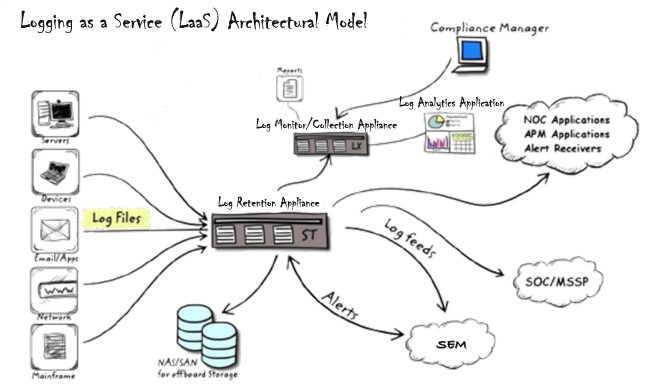
\includegraphics[width=0.80\textwidth]{images/Logging_as_a_Service_Architectural_Model}
        \caption[LaaS - Architektura]{
            LaaS - Architektura, źródło: \url{https://upload.wikimedia.org/wikipedia/commons/9/9c/Logging_as_a_Service_Architectural_Model.jpg}
        }
        \label{chapter:monitoring_architecture:laas:architecture_image}
    \end{figure}
    
    W tym wypadku wspomniany serwer zachowuje się
    jak baza danych. Jest to tak naprawdę jedna z jego funkcji. Poza tym specjalistyczne oprogramowanie na nim zainstalowane zajmuje się:
    \begin{itemize}
        \item normalizowaniem do wspólnego formatu,
        \item wizualizacją,
        \item analizą,
        \item raportowaniem wykrytych sytuacji wyjątkowych,
        \item archiwizacją,
        \item korelowaniem danych uzyskanych z analizy informacji pochodzących z innych źródeł.
    \end{itemize} \cite{laas_wikipedia}
    
    \subsection{Korzyści wynikają z LaaS}
    Ilość logów generowanych przez pojedynczą aplikację może sięgać tysięcy na minutę.
    Zapisywana jest każda ważniejsza akcja wykonana przez system. Przełączenie aplikacji
    w tryb debugowania\footnote{Tryb debugowania - w kontekście logowania jest to zakres informacji,
        które pojawią się w logach} spowoduje znaczący wzrost ilości danych.
    Dodatkowo sprawę komplikuje fakt, że większość dużych aplikacji tworzona jest w skalowalnej architekturze
    mikroserwisów. Innymi słowy składa się ona z wielu programów, z których każdy generuje własne logi i
    może się on znajdować na innej maszynie fizycznej lub wirtualnej.
    
    Bez rozwiązań typu \textbf{LaaS} administratorzy systemu czy też nawet programiści musieliby polegać
    na samych sobie. Konieczne byłoby ustalenie miejsca (serwera), na którym wystąpił problem, a w dalszej
    konieczności manualne przeszukanie plików logów. Wolumin danych byłby tutaj szczególnym utrudnieniem.
    Często aplikacja, w której zauważony zostałby problem, nie jest jego źródłem. W tym momencie konieczne
    jest przeanalizowanie kolejnych programów, znajdujących się wcześniej w procesie przetwarzania.
    \textbf{LaaS} efektywnie przeciwdziała temu problemowi poprzez agregowania logów we wspólnym miejscu,
    przez co analiza staje się łatwiejsza, a zaoszczędzony czas przekłada się na 
    szybszą implementacje nowych funkcjonalności oraz większy przychód dla firmy
    lub organizacji stojącej za produktem \cite{log_management_explained}. Z drugiej strony, dane dostępne
    są dla wielu, a nie jedynie dla wybranej garstki osób. Dzięki scentralizowaniu danych możliwe jest
    aby nie tylko programiści, ale także członkowie wsparcia technicznego mieli do nich dostęp.
    Przykłada się to na szybszą i lepszą analizę, a usuwanie usterki zajmuje mniej czasu. Problemy, zwłaszcza
    w skomplikowanych systemach, dotyczą więcej niż jednego poziomu aplikacji. Im krótsza będzie ścieżka,
    na końcu której znajdują się rozwiązania dla zaistniałej sytuacji, tym mniejsze straty firma poniesie.
    Z punktu widzenia właściciela, udziałowców mniejsza straty to większy zysk \cite{log_management_to_build_or_to_buy}.
    
    \subsection{Wady rozwiązań LaaS}
    Architektura oraz samo rozwiązanie LaaS, podobnie jak każde oprogramowanie, obarczone jest pewnymi
    wadami, które wynikają z jego natury. 
    
    \subsubsection{Wymagana nadmiarowość}
    \label{chapter:monitoring_architecture:laas:issue:data_size}
    LaaS wymaga wiele, szczególnie, przestrzeni dyskowej. Jest to związane z koniecznością zbierania logów z więcej niż jednego
    systemu do centralnej lokalizacji. Skala monitorowanych systemów przekłada się na ilość potrzebnego miejsca. Nadmienić trzeba, 
    że nie chodzi tutaj jedynie o ilość gigabajtów potrzebnych do zapisania tylko tego, co zostało przesłane. Nadmiarowość, w tym kontekście,
    odnosi się przede wszystkim do ciągłej dostępności tych danych - \textbf{HE}(\textit{high availability}). Aby spełnić ten wymóg
    konieczna staje się replikacja danych. Oczywistym minimum jest konfiguracja zakładająca jedną replikę, ale często dane, zwłaszcza te
    o wysokim znaczeniu, replikuje się na większą ilość serwerów. Tak więc ilość potrzebnej przestrzeni dyskowej
    rośnie liniowo, wraz ze zwiększaniem się ilości replik.
    
    Z drugiej strony, przechowywane dane nawet jeśli byłyby powielone na 100 serwerach, są bezużyteczne bez oprogramowania, które
    pozwoli uzyskać do nich dostęp. Jeśli monitorowany system jest duży, umieszczenie takiego programu na tylko jednym serwerze nie wystarczy.
    Konieczne jest zaprojektowanie klastra\footnote{Klaster - w technologi informatycznej to grupa serwerów, aplikacji działających równolegle, celem dostarczania wyniku.} takich aplikacji. 
    
    Wymienione zostały jedynie dwa elementy architektury \textbf{LaaS}. Oba z nich jednak wymagają kolejnego rodzaju maszyn, które koordynowałyby dostęp do nich.
    \textbf{Load-Balancer} to specjalny rodzaj oprogramowania, umieszczany przed aplikacjami docelowymi, którego zadaniem jest 
    rozdzielanie napływających zadań pomiędzy zarządzane maszyny, celem rozłożenia obciążania \cite{log_management_to_build_or_to_buy}.
    
    \subsubsection{Dłuższa retencja danych}
    Aby w pełni wykorzystać logi potrzebna jet dłuższa ich retencja. Jest to problem związany z koniecznością posiadania
    redundancji w przypadku przestrzeni dyskowej (\ref{chapter:monitoring_architecture:laas:issue:data_size}). 
    Retencja danych oznacza, że są one przechowywane przez pewien czas. Dla różnego rodzaju danych wymiar retencji
    może znacząco się różnić. Będzie on zależał od znaczenia zawartych w nich informacji. W przypadku logów
    kwestia ta wygląda podobnie, a różnice, często dosyć duże, będą w głównym stopniu wynikały z tego od jakiej
    aplikacji pochodzą logi oraz czy są one związane z bezpieczeństwem. Jeśli jednak pominąć znaczenie, które 
    tak naprawdę określane jest przez administratorów lub operatów wykorzystujących \textbf{LaaS}, konieczne jest
    zapewnienie, że dane, jeśli to wymagane, będą dostępne przez wymagany okres czasu. 